\documentclass{beamer}
\mode<presentation>
\usepackage{amsmath}
\usepackage{amssymb}
\usepackage{adjustbox}
\usepackage{subcaption}
\usepackage{enumitem}
\usepackage{multicol}
\usepackage{mathtools}
\usepackage{minted}
\usepackage{listings}
\usepackage{url}
\def\UrlBreaks{\do\/\do-}
\usetheme{Boadilla}
\usecolortheme{lily}
\setbeamertemplate{footline}
{
  \leavevmode%
  \hbox{%
  \begin{beamercolorbox}[wd=\paperwidth,ht=2.25ex,dp=1ex,right]{author in head/foot}%
    \insertframenumber{} / \inserttotalframenumber\hspace*{2ex} 
  \end{beamercolorbox}}%
  \vskip0pt%
}
\setbeamertemplate{navigation symbols}{}

\providecommand{\nCr}[2]{\,^{#1}C_{#2}} % nCr
\providecommand{\nPr}[2]{\,^{#1}P_{#2}} % nPr
\providecommand{\mbf}{\mathbf}
\providecommand{\pr}[1]{\ensuremath{\Pr\left(#1\right)}}
\providecommand{\qfunc}[1]{\ensuremath{Q\left(#1\right)}}
\providecommand{\sbrak}[1]{\ensuremath{{}\left[#1\right]}}
\providecommand{\lsbrak}[1]{\ensuremath{{}\left[#1\right.}}
\providecommand{\rsbrak}[1]{\ensuremath{{}\left.#1\right]}}
\providecommand{\brak}[1]{\ensuremath{\left(#1\right)}}
\providecommand{\lbrak}[1]{\ensuremath{\left(#1\right.}}
\providecommand{\rbrak}[1]{\ensuremath{\left.#1\right)}}
\providecommand{\cbrak}[1]{\ensuremath{\left\{#1\right\}}}
\providecommand{\lcbrak}[1]{\ensuremath{\left\{#1\right.}}
\providecommand{\rcbrak}[1]{\ensuremath{\left.#1\right\}}}
\theoremstyle{remark}
\newtheorem{rem}{Remark}
\newcommand{\sgn}{\mathop{\mathrm{sgn}}}
\providecommand{\abs}[1]{$\left\vert#1\right\vert$}
\providecommand{\res}[1]{\Res\displaylimits_{#1}} 
\providecommand{\norm}[1]{\lVert#1\rVert}
\providecommand{\mtx}[1]{\mathbf{#1}}
\providecommand{\mean}[1]{$E\left[ #1 \right]$}
\providecommand{\fourier}{\overset{\mathcal{F}}{ \rightleftharpoons}}
\providecommand{\system}{\overset{\mathcal{H}}{ \longleftrightarrow}}
\providecommand{\dec}[2]{\ensuremath{\overset{#1}{\underset{#2}{\gtrless}}}}
\newcommand{\myvec}[1]{\ensuremath{\begin{pmatrix}#1\end{pmatrix}}}
\let\vec\mathbf

\lstset{
frame=single, 
breaklines=true,
columns=fullflexible
}

\numberwithin{equation}{section}

\title{Collinearity of Points}
\author{Tarun Reddy Pakala \\ AI24BTECH11023}

\date{\today} 
\begin{document}

\begin{frame}
\titlepage
\end{frame}

\section{Problem}
\begin{frame}
\frametitle{Problem Statement}
Prove that the points \(\brak{2,-1,3}\), \(\brak{3,-5,1}\), and \(\brak{-1,11,9}\) are collinear using vectors.
\end{frame}

\section{Solution}
\begin{frame}
\frametitle{Solution}
Let \( A = \brak{2, -1, 3} \), \( B = \brak{3, -5, 1} \), and \( C = \brak{-1, 11, 9} \).

Construct the vectors:
\[
\overrightarrow{B-A} = \brak{3-2, -5+1, 1-3} = \brak{1, -4, -2}
\]
\[
\overrightarrow{C-A} = \brak{-1-2, 11+1, 9-3} = \brak{-3, 12, 6}
\]
\end{frame}

\begin{frame}
\frametitle{Matrix Representation}
Next, we construct the matrix using these vectors:
\[
\text{Matrix} = 
\begin{pmatrix}
\overrightarrow{B-A} & \overrightarrow{C-A}
\end{pmatrix}
= 
\begin{pmatrix}
1 & -3 \\
-4 & 12 \\
-2 & 6
\end{pmatrix}
\]
\end{frame}

\begin{frame}
\frametitle{Row Reduction}
Now, we perform row reduction:
\[
\begin{pmatrix}
1 & -3 \\
-4 & 12 \\
-2 & 6
\end{pmatrix}
\rightarrow
\begin{pmatrix}
1 & -3 \\
0 & 0 \\
0 & 0
\end{pmatrix}
\]
Since the matrix has rank 1 (only one non-zero row), the points are collinear.
\end{frame}

\begin{frame}[fragile]
\frametitle{C-Code}
\begin{minted}[bgcolor=bg, linenos, fontsize=\small, breaklines]{c}
    #include <stdio.h>

int main() {
    // Define points
    double points[3][3] = {
        {2.0, -1.0, 3.0},
        {3.0, -5.0, 1.0},
        {-1.0, 11.0, 9.0}
    };

    // Open file for writing
    FILE *file = fopen("points.txt", "w");
    if (file == NULL) {
        return 1;  // Exit if file cannot be opened
    }
\end{minted}
\end{frame}
\begin{frame}[fragile]
\frametitle{C-Code}
\begin{minted}[bgcolor=bg, linenos, fontsize=\small, breaklines]{c}
  // Write points to the file
    for (int i = 0; i < 3; i++) {
        fprintf(file, "%lf %lf %lf\n", points[i][0], points[i][1], points[i][2]);
    }

    fclose(file);
    return 0;
}
\end{minted}
\end{frame}
\begin{frame}
\frametitle{C-Code Output}
2.000000 -1.000000 3.000000 \\\\
3.000000 -5.000000 1.000000 \\\\
-1.000000 11.000000 9.000000 
\end{frame}

\begin{frame}[fragile]
\frametitle{Python Code}
\begin{minted}[bgcolor=bg, linenos, fontsize=\small, breaklines]{python}
import matplotlib.pyplot as plt
from mpl_toolkits.mplot3d import Axes3D

# Read points from the file
points = []
with open("points.txt", "r") as file:
    for line in file:
        # Remove parentheses and split by commas
        point = line.strip()[1:-1].split(", ")
        points.append([float(coord) for coord in point])

# Convert points to a numpy array for easier handling
points = list(zip(*points))  # Unzips the list of points

# Create a 3D plot
fig = plt.figure()
ax = fig.add_subplot(111, projection='3d')
\end{minted}
\end{frame}

\begin{frame}[fragile]
\frametitle{Python Code}
\begin{minted}[bgcolor=bg, linenos, fontsize=\small, breaklines]{python}
# Plot the points
ax.scatter(points[0], points[1], points[2], color='red', s=100)

# Connect the points with a line
ax.plot(points[0], points[1], points[2], color='blue')

# Annotate the points
for i, point in enumerate(zip(*points)):
    ax.text(point[0], point[1], point[2], f'P{i+1} {point}', size=10, zorder=1)

# Set labels
ax.set_xlabel('X')
ax.set_ylabel('Y')
ax.set_zlabel('Z')
ax.set_title('3D Plot of Points')
# Show the plot
plt.show()
\end{minted}
\end{frame}


\section{Graphical Representation}
\begin{frame}{Graphical Representation}
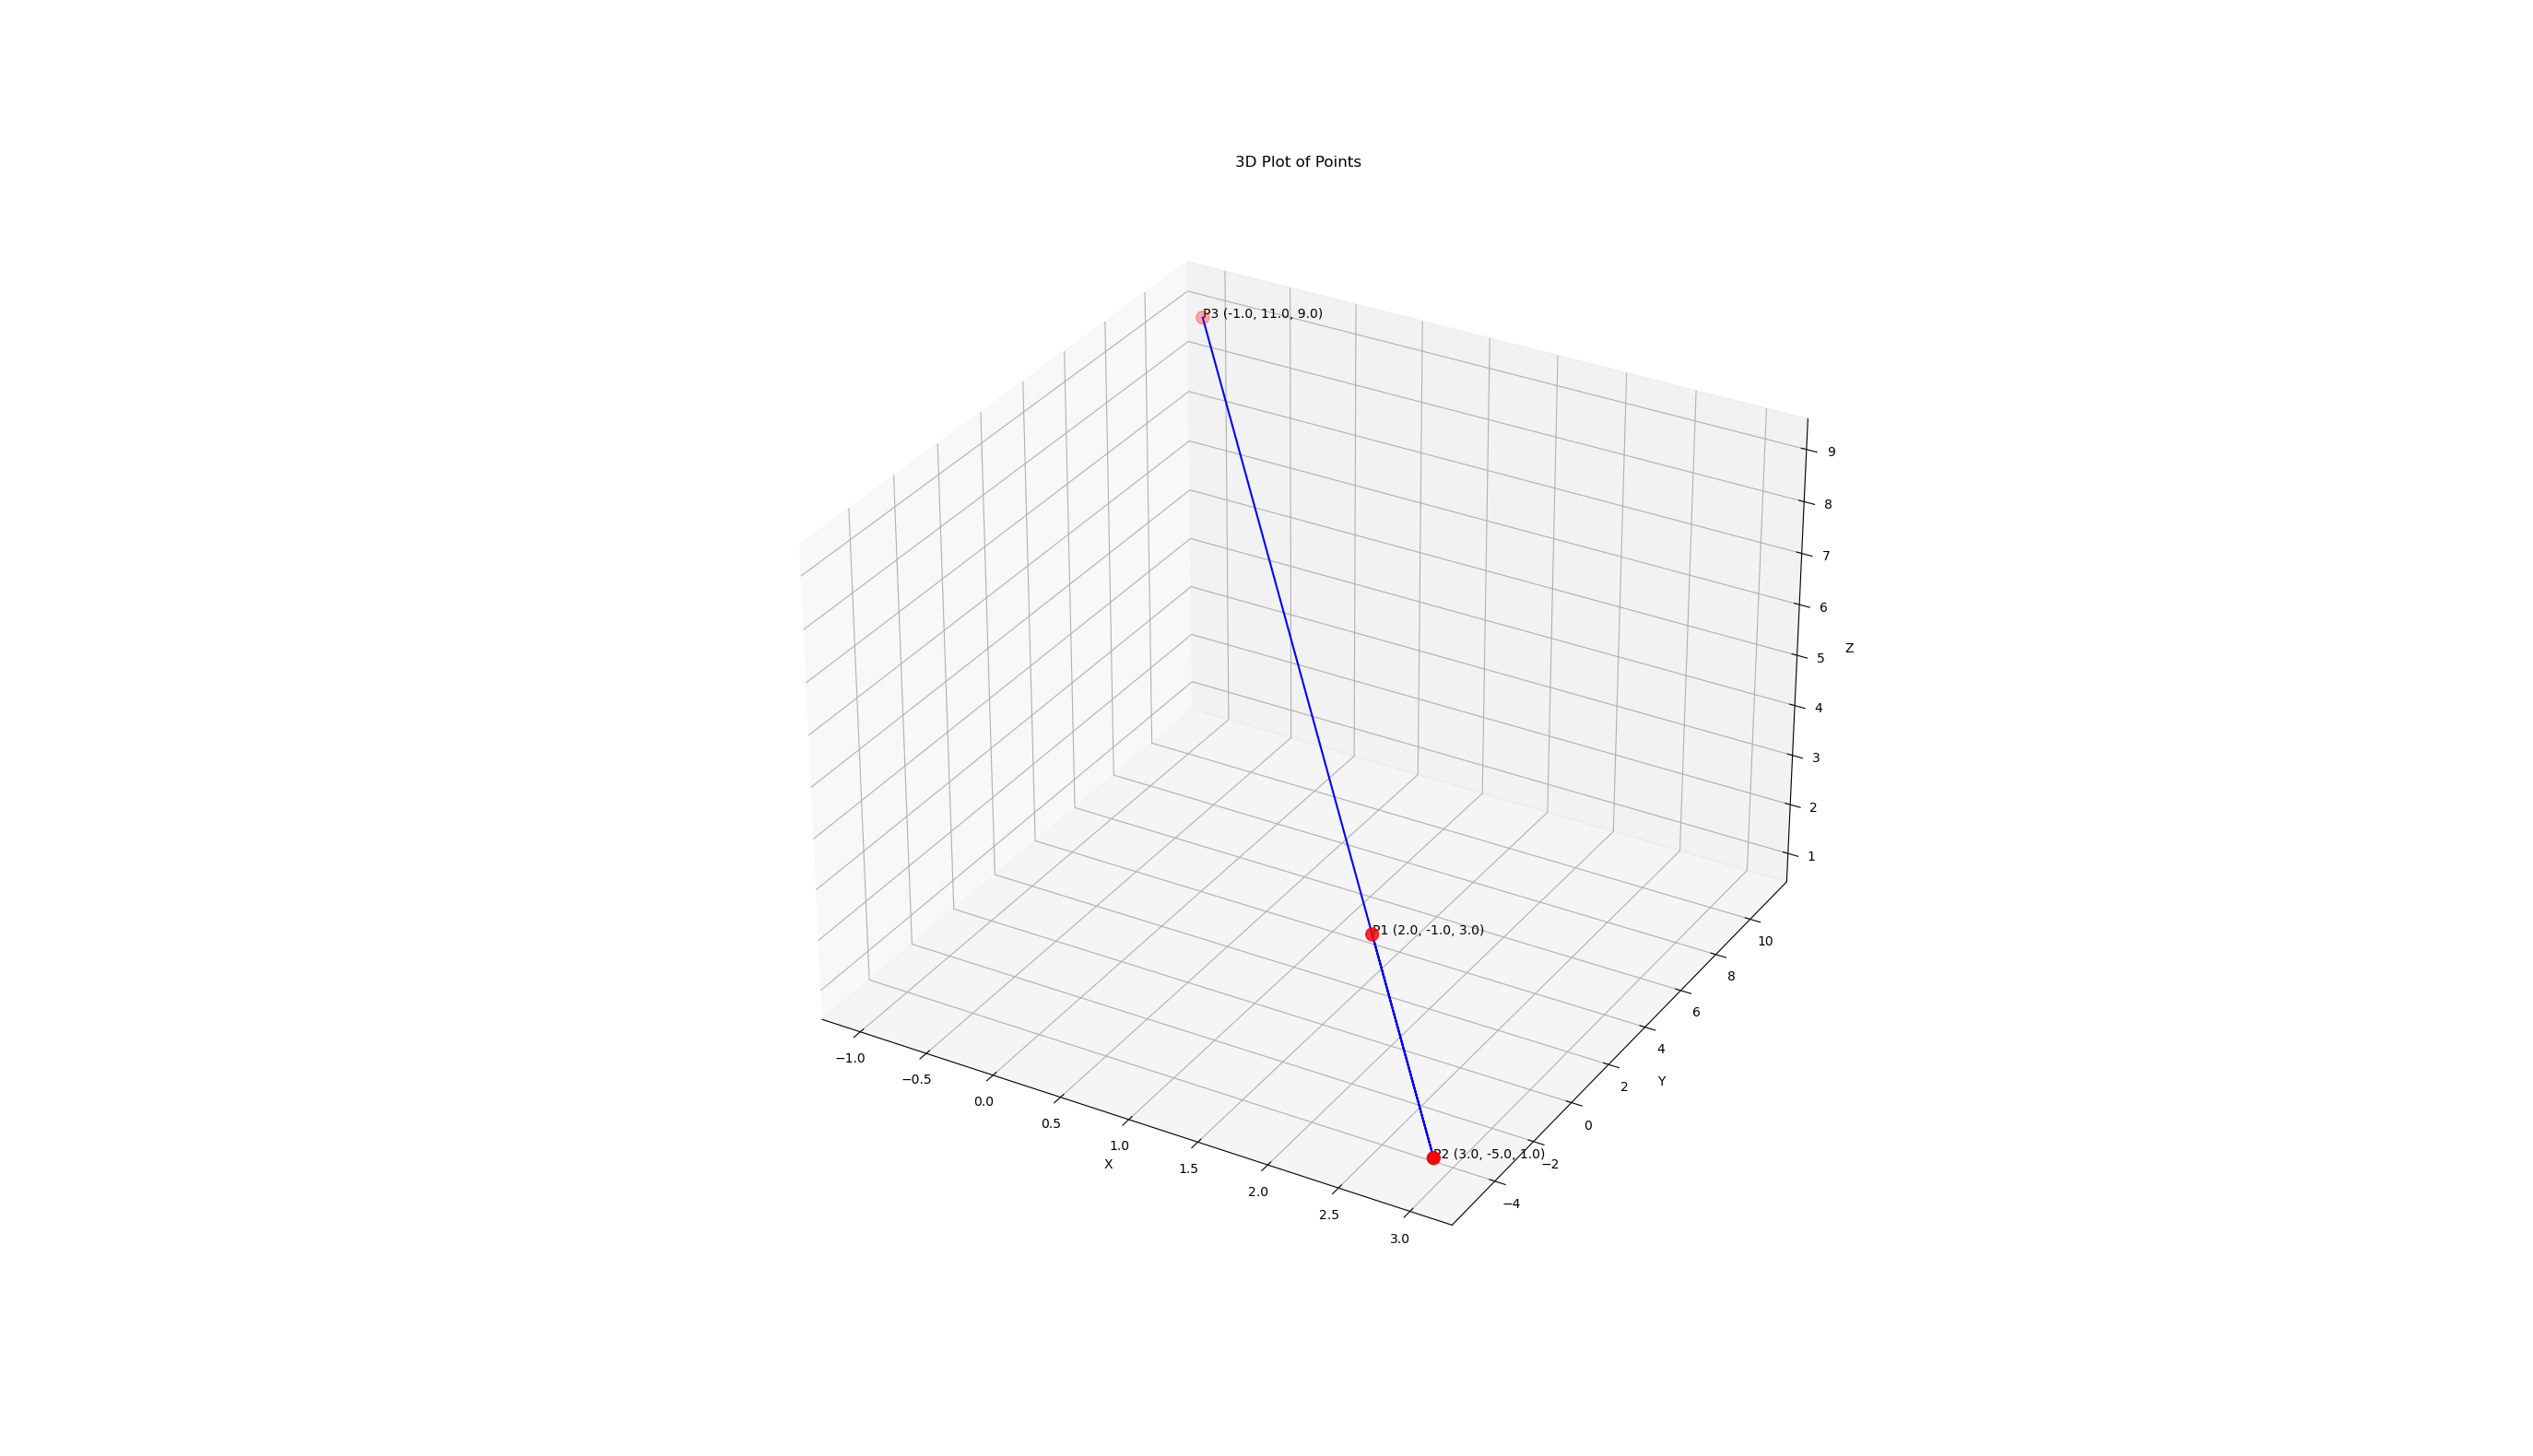
\includegraphics[width=1\textwidth]{Figure_1.png}

\end{frame}
\section{Conclusion}
\begin{frame}
\frametitle{Conclusion}
The points \(\brak{2,-1,3}\), \(\brak{3,-5,1}\), and \(\brak{-1,11,9}\) are confirmed to be collinear based on the row reduction of the constructed matrix.
\end{frame}

\end{document}

